

%%%%%%%%%%%%%%%%%%%%%%%%%%%%%%%%%%%%%%%%%%%%%%%%%%%%%%%%%%%%%%%%%%%%%%%%%%%%%%%%%%%%%%%%%%%%%%%%%%%
\chapter{Forks e ataques de 51\%}
%\label{ch:chapter6}

%\paragraph{}

No início, Satoshi minerou os primeiros bitcoins usando a unidade de processamento central (CPU) do computador.
Como a dificuldade inicial de mineração no sistema era baixa, era relativamente barato gerar essas moedas usando a CPU.

Com o tempo, as pessoas começaram a ajustar o software de mineração para torná-lo cada vez mais eficiente.
Eventualmente, eles escreveram um software que começou a tirar proveito de processadores especializados chamados unidades de processamento gráfico (GPUs) que existem nas placas de vídeo e geralmente são usados para jogos.

%adaptado
Com as GPUs, a mineração tornou-se milhares de vezes mais eficiente do que a mineração usando a CPU.
A dificuldade rapidamente se ajustou para cima para equivaler ao novo taxa de Hash que havia enchido a rede pelo uso de GPUs.
Nesse ponto, qualquer pessoa que minerava em uma CPU fornecia uma fração tão pequena da taxa de hash que rapidamente se tornou não lucrativo e tiveram que desligar seus mineradores.
%, pois a dificuldade aumentou devido a todos os novos mineradores de GPU.

Conforme as GPUs assumiram o controle e as pessoas começaram a comprar toneladas de placas gráficas, a eficiência da mineração foi aprimorada ainda mais por meio da produção de ASICs (Application Specific Integrated Circuits, ou Circuitos Integrados Específicos de Aplicações em português).
São chips de hardware de computador que são criados com um objetivo específico - a função bitcoin sha256 e nada mais. 
Sendo especializados neste algoritmo em particular, os ASICs foram capazes de ser milhares de vezes mais eficientes do que as GPUs para mineração e rapidamente tornaram as GPUs não lucrativas, assim como as GPUs fizeram com as CPUs.
Em poucos anos, a nova geração de dispositivos ASIC coloca suas versões anteriores fora do mercado com grandes melhorias de eficiência.

Os primeiros mineradores da rede gastaram apenas alguns centavos de eletricidade para produzir seus bitcoins. 
À medida que o preço do bitcoin subia e mais e mais mineradores aderiam a rede, a dificuldade aumentava e ficava cada vez mais caro gerar bitcoins. 
Hoje, o preço gira em torno de \$ 8000.00 por moeda, e pessoas queimam milhares de reais em eletricidade por unidade de bitcoin criado.

\section*{Pools de mineração}

Um problema com a mineração de bitcoin é que ela não é determinística, como jogar um dado. 
Isso significa que você pode acabar gastando centenas de dólares em eletricidade e nunca encontrar um bloco válido.

Em 2010, uma inovação chamada pool de mineração (conhecida como Slushpool) surgiu para resolver o problema de mineradores consumindo energia sem receber recompensa.
Um pool de mineração é um pool de risco compartilhado, semelhante ao funcionamento do seguro médico.

Todos os mineradores contribuem com a mineração, fazendo com que todos os participantes pareçam um grande minerador.
Se alguém na pool encontrar um bloco válido, a recompensa pelo bloco é dividida proporcionalmente entre todos os mineradores com base na taxa de hash com que contribuíram.
Isso permite que até mesmo pequenas operações de mineração, como indivíduos, recebam recompensa pela pequena taxa de hash com que contribuem. 
Para fornecer este serviço de coordenação, o pool fica com uma parte das recompensas.

% Além disso, não devemos presumir que, apenas porque um pool de mineração tem uma porcentagem específica de taxa de hash, eles possuem o hardware.
% Na verdade, a maioria das pools de mineração é composta por milhares de mineradores individuais. 
% Se o pool de mineração começar a se comportar mal, esses mineradores teriam um incentivo para sair do pool porque gostariam de proteger o valor econômico do Bitcoin, que estão minerando presumivelmente para ganhar dinheiro e não para ter prejuízos!



%adicionado
Os pools de mineração causaram um efeito de centralização, os usuários tendem a migrar para pools maiores.
Porem, é importante lembrar que usuários estão minerando para a pool e que a pool não é detentora da taxa de hash que eles representam. 
Usuários podem trocar de pool de mineração ao longo do tempo e fazem isso.
O diagrama abaixo mostra a distribuição aproximada da mineração em janeiro de 2019.

\begin{figure}
  \centering
  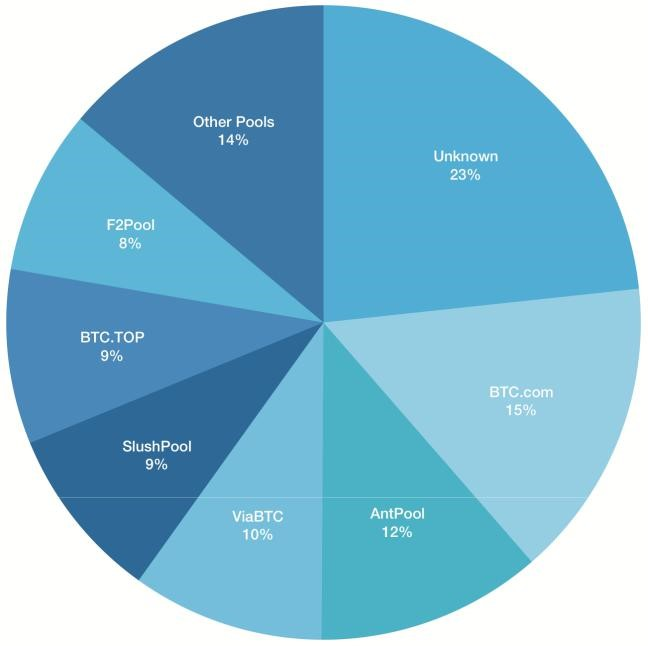
\includegraphics[width=7cm]{imagens/capitulo-9-pizza.jpg}
  \caption*{\textit{\small Pools de mineração}}
\end{figure}

%reposicionado
Na verdade, há um precedente histórico para mineradores individuais deixarem uma pool que se tornou muito poderosa: em 2014, a Ghash.io tinha quase metade do poder de mineração total. 
Os mineiros viram que ele estava se tornando muito centralizada e partiram para outras pools de maneira voluntaria.

%reposicionado
Embora pools de mineração relativamente centralizadas sejam a realidade atual, há melhorias constantes na tecnologia de mineração, incluindo uma proposta chamada BetterHash, que permite que os mineradores individuais tenham mais controle sobre o que estão minerando e reduza a dependência da coordenação das pools.



\section*{Ataques de 51\%}
%\paragraph{}

A centralização do pool de mineração leva à preocupação de que eles possam conspirar para o ataque de 51\% da rede.
Se você olhar o gráfico acima, verá que as 5 principais pools, em conjunto, têm mais de 50\% da taxa de hash de mineração total.
Vamos examinar como esse ataque é realizado e quais perigos ele carrega.

Quando você possui pouco mais de 50\% da taxa de hash, pode dominar as gravações no livro-razão porque pode produzir uma cadeia mais longa do que a outra taxa de hash inferior a 50\% combinada ao longo do tempo.
Lembre-se de que o Consenso de Nakamoto diz que os nodes devem aceitar a cadeia de Prova de Trabalho cumulativa mais longa que chegar até eles.


Aqui está um exemplo de como um ataque simples de 51\% é realizado:

\begin{enumerate}
\item Digamos que a rede como um todo esteja produzindo 1000 hashes/segundo;
\item Você compra um monte de hardware de mineração e eletricidade para produzir 2.000 hashes/segundo. Agora você tem 66\% da taxa total de hash (2000/3000);
\item Você começa a minerar uma cadeia que contém apenas blocos vazios;
\item Daqui a duas semanas, você transmitirá sua blockchain vazia. Como você está minerando aproximadamente duas vezes mais rápido que os mineradores honestos, sua cadeia será duas vezes mais longa focando na Prova de Trabalho cumulativa.
A transmissão para todos os nodes existentes fará com que eles se reorganizem e percam as últimas duas semanas de história escrita na blockchain.
\end{enumerate}

Além de minerar blocos vazios, o que torna a blockchain inutilizável, você também pode realizar um ataque de gasto duplo:

\begin{enumerate}
\item Envie algum bitcoin para uma exchange;
\item Troque por USD e retire o USD;
\item Mais tarde, transmita na blockchain que você minerou secretamente e que não contém o envio para a exchange;
\item Você reescreveu a história e agora tem o bitcoin original e os dólares;
\end{enumerate}

%modificado
Com o consumo de energia da taxa de hash do Bitcoin hoje sendo mais ou menos a de um pais de médio porte. %(lembre-se, ele está usando a mesma quantidade de energia de um país de porte médio) 
Adquirir hardware e eletricidade suficientes para realizar tal ataque é extremamente caro.
Estimativas mostram que custaria para você aproximadamente \$700k Dólares por hora para realizar um ataque de 51\% hoje, e o custo continua a subir. 
Essa estimativa não leva em conta a reação que mineradores honestos terão ao a tal ataque, que a tudo indica fariam ele custar ainda mais. Você pode explorar o custo de um ataque ao Bitcoin ou outras criptomoedas em \url{https://www.crypto51.app}.

Também é muito difícil escapar impune com um ataque de gasto duplo dessa proporção sem deixar pegadas que poderiam ser usadas para descobrir quem você é. 
Afinal, você estaria consumindo a energia de um país de porte médio e comprando milhões de dólares em hardware e enviando milhões de dólares para a exchange para fazer todo este processo.

Manter esse tipo de ataque por qualquer período de tempo razoável é inviável, mas digamos que uma entidade mal-intencionada com financiamento ilimitado decidisse fazer isso e fosse capaz de sustentar esse ataque além do nível de um incômodo.
A rede poderia se adaptar alterando a sua função de prova de trabalho (usando alguma coisa diferente do sha256).
Isso tornaria todos os ASICs de hardware usados pelo invasor completamente inúteis. 
Essa, no entanto, é a opção nuclear, pois também tiraria do mercado imediatamente todos os mineradores honestos.No entanto, a rede sobreviveria e surgiria das cinzas, como a Fênix.

Além da inviabilidade do ataque, ter a maioria da taxa de hash não dá direito a ser dono da rede:

\begin{enumerate}
\item Você não pode criar moedas do nada. Isso viola a regra de consenso de recompensa de blocos, sendo eles rejeitados, mesmo se tivessem Prova de Trabalho suficiente;
\item Você não pode gastar moedas que não são suas. Você não seria capaz de fornecer uma assinatura digital válida, o que viola as regras;
%\item Você não pode acelerar o cronograma de emissão de Bitcoin. A dificuldade seria ajustada a cada 2016 blocos como sempre faz.
\end{enumerate}

%modificado
Assim, os nodes que aceitam Bitcoin como pagamento manteriam a rede honesta mesmo em face de uma maioria desonesta de mineradores, simplesmente seguindo as regras do Bitcoin.
Portanto, um ataque de 51\% é mais um incomodo do que um problema de segurança.
O mais provável, pior cenário possível aqui seria um estado, que possui bolso fundo que esteja tentando tornar o bitcoin não utilizável.
No entanto tal ataque não pode se manter por muito tempo.
Quando o Bitcoin se recuperar de um ataque como esse apenas provaria a resiliência e tornaria o bitcoin um problema ainda maior para aqueles que desejam atacar ele.

Enquanto ate a presente data o Bitcoin nunca foi realizado um ataque de 51\% com sucesso, o ataque já foi realizado em outras \textit{blockchains} que possuem taxa de hash pequena protegendo elas.
Nestes casos, exchanges foram vitimas de ataques de gasto-duplo e perderam dinheiro nessas moedas de pouca taxa de hash, que eles provavelmente não deveriam ter listado em primeiro lugar.

